\documentclass[12pt]{article}
\usepackage{amssymb,latexsym,amsmath}
%\usepackage{epsfig}
%\usepackage{graphicx}  
%\DeclareGraphicsExtensions{.pdf, .jpg, .tif, .eps, .jpg}

\newif\ifpdf
\ifx\pdfoutput\undefined
\pdffalse % we are not running PDFLaTeX                                        
\else
\pdfoutput=1 % we are running PDFLaTeX                                         
\pdftrue
\fi
\ifpdf
\usepackage[pdftex]{graphicx}
\else
\usepackage{graphicx}
\fi
\ifpdf
\DeclareGraphicsExtensions{.pdf, .jpg, .tif}
\else
\DeclareGraphicsExtensions{.eps, .jpg}
\fi



\textwidth = 6.5 in
\textheight = 9 in
\oddsidemargin = 0.0 in
\evensidemargin = 0.0 in
\topmargin = -0.5 in
\headheight = 0.0 in
\headsep = 0.0 in
\parskip = 0.2 in
\parindent = 0.0 in


%%%%%%%%%%%%%%%%%%%%%%%%%%%%%%%%%%%%%%%%%%%%%%%%%%%%%%%%%%%%%%%%%%%%%%%%


\newcommand{\khat}{\hat{\mathbf k}}
\newcommand{\uv}{\mathbf u}
%\newcommand{\omegav}{\mathbf \omega}
\newcommand{\omegav}{\mathbf w}
\newcommand{\w}{\mathbf w}
\newcommand{\grad}{\nabla}
\newcommand{\curl}{\grad \times}

\DeclareMathOperator{\Span}{span}


\title{The Boussinesq equations and Coordinate scalings in the
  LANL-Sandia DNS code} \author{Mark Taylor, Beth Wingate, Susan Kurien}

\begin{document}
\maketitle

\section{Scaling of the Domain}


\begin{figure}
\begin{center}
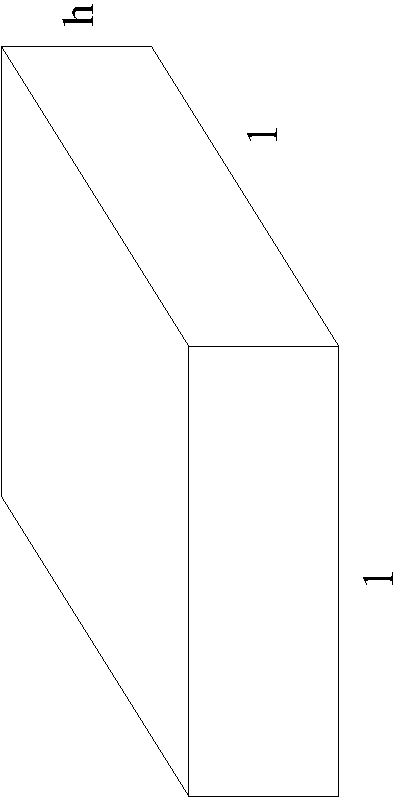
\includegraphics[angle=-90,width=4.in]{box}
\caption{ }
\label{F:box}
\end{center}
\end{figure}



We would like to solve the NS equations in the box pictured in
Fig.~\ref{F:box}.  The equations are
\[
\frac{ \partial  \uv }{\partial t}  + (\curl \uv + f \khat) \times \uv + 
\grad \pi + N \theta \khat = \nu \Delta \uv
\]
\[
\grad \cdot \uv = 0
\]
\[
\frac{ \partial  \theta }{\partial t}  + \uv \cdot \grad \theta - 
N \uv \cdot \khat = \kappa \Delta \theta
\]
The Schmidt number is $\nu / \kappa$.  

We refer to the coordinate system in the box in Fig.~\ref{F:box} as
the primted coordinate system, and we now introduce a 
change of variables, into the {\em non-primed} coordinate
system.  In the non-primed coordinate system, the domain because a 
unit cube:
\[
x = x', \qquad y=y', \qquad  z = \frac{z'}{h},
\]
The only change to our code is that:
\[
\frac{\partial}{\partial z'} = \frac{1}{h} \frac{\partial}{\partial z}
\]
And thus 
\[
\grad = 
\begin{pmatrix} \dfrac{\partial}{\partial x} \\[5mm]
                \dfrac{\partial}{\partial y} \\[5mm]
                \dfrac{1}{h} \dfrac{\partial}{\partial z} 
\end{pmatrix}
 \qquad
\Delta  = \left(\frac{\partial}{\partial x}\right)^2 + 
           \left(\frac{\partial}{\partial y}\right)^2 +
           \left(\frac{1}{h}\frac{\partial}{\partial z}\right)^2 
\]
and
\[
\grad \cdot \uv = \frac{\partial u_1 }{\partial x} + 
\frac{\partial u_2 }{\partial y} + 
\frac{1}{h} \frac{\partial u_3 }{\partial z}
\]
and  vorticity $\omegav$ is given by
\begin{equation}
\label{E:vor}
\omegav = \curl \uv = 
\begin{pmatrix}
\dfrac{\partial u_3}{\partial y} - \dfrac{1}{h} \dfrac{\partial u_2}{\partial z}  \\[5mm]
\dfrac{1}{h} \dfrac{\partial u_1}{\partial z} -  \dfrac{\partial u_3}{\partial x}  \\[5mm]
\dfrac{\partial u_2}{\partial x} - \dfrac{\partial u_1}{\partial y}
\end{pmatrix}  
\end{equation}


The divergence free condition on $\uv$ is solved by the choice
of $\pi$.  This involves, 
for some vector field ${\mathbf v}$, 
solving an equation of the form 
\[
\Delta \pi = \grad \cdot {\mathbf v}
\] 
The remaining equations we write in component form:
\[
\begin{pmatrix} u_1 \\
                u_2 \\
                u_3 \\
\end{pmatrix}_t
  + (\omegav + f \khat) \times 
\begin{pmatrix} u_1 \\
                u_2 \\
                u_3 \\
\end{pmatrix}
+ \grad \pi +
\begin{pmatrix} 0 \\
                0 \\
                N \theta \\
\end{pmatrix}
= \nu 
\begin{pmatrix} \dfrac{\partial^2 u_1}{\partial x^2} + 
                \dfrac{\partial^2 u_1}{\partial y^2} + 
                \dfrac{1}{h^2}\dfrac{\partial^2 u_1}{\partial z^2}   \\[5mm]
                \dfrac{\partial^2 u_2}{\partial x^2} + 
                \dfrac{\partial^2 u_2}{\partial y^2} + 
                \dfrac{1}{h^2}\dfrac{\partial^2 u_2}{\partial z^2}   \\[5mm]
                \dfrac{\partial^2 u_3}{\partial x^2} + 
                \dfrac{\partial^2 u_3}{\partial y^2} + 
                \dfrac{1}{h^2}\dfrac{\partial^2 u_3}{\partial z^2}
\end{pmatrix}
\]
\[
\frac{ \partial  \theta }{\partial t}  + \uv \cdot \grad \theta - 
N u_3  = \kappa \left(
                \dfrac{\partial^2 \theta}{\partial x^2} + 
                \dfrac{\partial^2 \theta}{\partial y^2} + 
                \dfrac{1}{h^2}\dfrac{\partial^2 \theta}{\partial z^2}
\right)
\]



Thus the only changes needed for our parallel DNS code are is that
all derivatives in $z$ need to be scaled by $h$.


\section{Hyper Viscosity}
Consider our scaled hyper viscosity term
\[
\frac{ \partial  \uv }{\partial t} = 
\sqrt{E(k_\textrm{max})} \,  k_\textrm{max}^{-2\eta + 1.5}  \Delta^\eta \uv
\]
We first verify that the units are correct.  The units of
energy are $m^2/s^2$, so the units of the energy in a single
spherical shell $E(k)$ is $m^3/s^2$.  Thus we have
\[
\frac{m}{s^2} = \frac{m^{1.5}}{s} \,\frac{1}{m^{-2\eta+1.5}}  
                          \,\frac{1}{m^{2\eta}}
                           \, \frac{m}{s}
\]
In the frequency domain, 
\[
\frac{ \partial  u_3 }{\partial t} = 
\sqrt{E(k_\textrm{max})} \,  k_\textrm{max}^{-2\eta + 1.5}  
( (2\pi l)^2 + (2\pi m)^2 + (2\pi n/h)^2)^\eta u_3
\]

\section{Resolution Condition}

The assumptions made in the hydrostatic equations implicitly assume
(acording to Leslie) that 
\[
 \max{ k_h } << \min{k_z}
\]
which works out to (assuming 2/3 dealiasing)
\[
   \frac{N_x}{3} <<  \frac{1}{h}
\]



\section{Computing Scalars}
Integrals per unit volume are approximated by the sum
\[
<f,g> = \frac{1}{h} \iiint  f g  \, dx' \, dy' \, dz' =   \iiint  f g \, dx \, dy \, dz
=\frac{1}{N_x N_y N_z} \sum  f  g
\]
We also have that 
\[
\frac{1}{N_x N_y N_z} \sum  f  g = \sum \hat{f} \hat{g}
\]
so integrals can be computed in Fourier or grid space. 

All other scalars (kinetic energy, helicity, various dissipation
terms) are computed in physical coordinates.  So for example
\[
k = <\uv,\uv> = <u_1,u_1> + <u_2,u_2> +  <u_3,u_3>
\]
and the helicity 
\[
  h  = w_1 u_1  + w_2 u_2 + w_3 u_3
\]
As in example, using integer wave numbers $(l,m,n)$ (defined in the
next section), we have
\[
< \omegav , \Delta \uv> = \sum (2 \pi)^2 (l^2 + m^2 + (n/h)^2) 
\, \uv \cdot \omegav
\]





\section{Computing 3D Energy Spectra (in a spherical shell)}
If we choose to discretize our domain so that the 
maximum wave number (in the primed coordinate system) is
the same in all diretions, then
\[
\Delta x' = \Delta y' = \Delta z'
\]
Or
\[
N_x  = N_y = N_z/h
\]
where $N_x$ is the number of grid points in the $x$ direction.
The highest wave number is given by:
\[
k_x = \pi N_x, \qquad k_y = \pi N_y, \qquad k_z = \pi N_z/h 
\]
(Note that $\pi$ appears in the wave numbers since our domain is
of length 1 in the $x$ and $y$ diretions.)  The wave number spacing
is given by
\[
\Delta k_x = 2 \pi, \qquad  \Delta k_y = 2 \pi, \qquad  \Delta k_z = 2 \pi / h 
\]
In our DNS code, we index our arrays of Fourier coefficients
with integers $(l,m,n)$, with $l=0 \dots N_x/2$, 
$m=0 \dots N_y/2$ and 
$n=0 \dots N_z/2$.  The wave number spacing is given by
given by
\[
k_x = l \Delta k_x,, \qquad  k_y = m \Delta k_y, \qquad  k_z = n  \Delta k_z
\]
We index the arrays containing power spectra
such as $E(k)$ with integer wave number $k$, represents a shell or anulus
of some chosen thickness centered around the wave number associated
with $k$.

The total energy is
\[
E  = \sum_{l,m,n}  |  {\hat u_1}(l,m,n) |^2 +
 |  {\hat u_2}(l,m,n) |^2 + 
 |  {\hat u_3}(l,m,n) |^2
\]

The standard energy spectrum is now, for integers $k$:
\[
E(k)  = \sum_{l,m,n}  |  {\hat u_1}(l,m,n) |^2 +
 |  {\hat u_2}(l,m,n) |^2 + 
 |  {\hat u_3}(l,m,n) |^2
\]
where the sum is taken over all integers $(l,m,n)$ such that
\[
(\Delta k_z)^2 (k-1/2)^2 \le (\Delta k_x l)^2 + (\Delta k_y m)^2 + (\Delta k_z n)^2 <  (\Delta k_z)^2 (k+1/2)^2 
\]
where we have chosen to use a shell thickness of $\Delta k_z$.
Scaling out the $2\pi$, we get
\[
(k-1/2)^2 \le  h^2 \left( l^2 + m^2 + (n/h)^2 \right) < (k+1/2)^2
\]  





\section{Computing 2D Energy Spectra (in an annulus)}
We also compute a 2D spectra $E(k_h,k_z)$ by summing squares of Fourier
coefficients over annular regions in 
$x$ and $y$ of radius $k_h$.  
where 
\[
k_h = \sqrt{(k_x^2 + k_y^2)} = \sqrt{(2\pi l)^2 + (2\pi m)^2}. 
\]
From this quantity, we can get $E(k_h,0)$, which 
represents the energy spectrum of the 2D field
obtained by averaging the original 3D field  in the direction of rotation,
and then summing the energy within spherical shells (an annulus for 2D fields).
We are also interested in 
\begin{equation}
E(k_h) = \sum_{k_z=0}^{\pi N_z/h} E(k_h,k_z) 
\label{E:SPECb}
\end{equation}
which represents 
the energy spectrum of the full 3D field, but summed over
the annular region between concentric cylinders
(whose axis are in the $z$ direction).  As with the spherical
shell spectrum, Eq.~\ref{E:SPECb} has the property that
it partitions the energy into a set of discrete wave numbers, so
that the total energy 
\[
E = \sum_{k_h} E(k_h)
\]


The 2D shell (annulus) thickness is now
determined by the horizontal wavenumber spacings. In our code,
we use an integer index $k$ defined by $k_h = k \Delta k_x$ and
define
\begin{eqnarray*}
E(k,j) = \sum_{l,m}  |  {\hat u_1}(l,m,n) |^2 +
 |  {\hat u_2}(l,m,n) |^2 + 
 |  {\hat u_3}(l,m,n) |^2
\end{eqnarray*}
where the sum is taken over fixed $n$ and all integers $(l,m)$ such that 
\[
(\Delta k_h)^2 (j-1/2)^2 \le (\Delta k_x l)^2 + (\Delta k_y m)^2  <  (\Delta k_h)^2 (j+1/2)^2 
\]
and with $k_x=k \Delta k_x$ for integers $k$.  
we have chosen to use a shell thickness of $\Delta k_h =\Delta k_x = \Delta
k_y = 2\pi$. Scaling out the $2\pi$, we get
\[
(j-1/2)^2 \le  l^2 +  m^2 < (j+1/2)^2.
\]  

\section{Running the Model for the Boussinesq equations}

\noindent
This section discusses important elements of the inputfile and how to
build the executable.

When you've chosen scalar type = 4 in the gridsetup script (see
below), you need to add a line to the input file right after the line
for the smagorinsky coefficient,
\noindent
\begin{verbatim}
.
.
.
107.08        ! Bous. parameter  Fr = .21/bous=107.08
0e0           ! alpha (for NS-alpha model).  alpha>1 is in units of delx
.0            ! smagorinsky
1             ! max number of schmidt numbers for passive scalars
1. 4          ! schmidt number = nu/kappa, ratio of viscous coeffs,type of scalar
0             ! compute_structure_functions
.
.
. 
\end{verbatim}


Note that the type in this file must match the type in the gridsetup
command. Also note that if you want to the code to compute the
two-point correlations of potential vorticity then you need to set the
value of \texttt{compute structure functions} to 1.

\noindent
To set up the model you need to use the following:

\begin{description}
  
\item[1)] Example to set the FORTRAN arrays sizes before compiling:
  ($32^3$ simulation on 8 processors, prognostic variables: $u,v,w$
  and $\theta$). Note the 4 on the end, which
  indicates the type of scalar equations for the code to use \\
 
  \begin{verbatim}
      ./gridsetup.py 1 1 8 32 32 32 2 2 2 0 0 0 4
  \end{verbatim}

  \noindent
  This one sets up the problem for $128^3$ on 32 processors
  like this:

  \begin{verbatim}
   ./gridsetup.py 1 1 32 128 128 128 2 2 2 0 0 0 4
  \end{verbatim}

\item[2)] Then one makes the Boussinesq equations by
  typing\\

  \begin{verbatim}
  gmake dnsb
  \end{verbatim}
  
\end{description}

\noindent

\section{Comparing with Smith \& Waleffe (SW99 and SW02)}

\subsection{Scalings and definitions}

\subsubsection*{$\underline{\text{Wave numbers}}$}
Wave numbers are dimensional and should be computed $k_f = 2 \pi
k_f^m$, where the superscript $m$ stands for Mark. 

\subsubsection*{$\underline{\text{Rossby Number}}$}
SW02 computes this Rossby number,
\begin{equation}
  Ro = \frac{(k_f^2 \epsilon_f)^{1/3}}{\text{fcor}/2}, 
\end{equation}
where each number in the equation is computed as,
\begin{description}
   \item[1)] $k_f = 2 \pi k_f^m$
   \item[2)] $\epsilon_f$ is computed as an average through the run using
     scalars.m. It can also be found for each time in the output file
     if one looks at the $d/dt$ line and hunts for the f parameter (for
     the forcing).
  \item[3)] fcor is an input to the code. There is some question as to
    whether we should divide by $fcor/2$ or $fcor$, see SW02 Eq 3.2

\end{description}

\subsubsection*{$\underline{\text{Froude number}}$}

Modifications to the dns code to accomodate this is to include the
addition of a parameter {\bf{bous}} which multiplies the vertical
velocity in the  density anomoly equation. The equations we actually
solve in the code are,
We would like to solve the NS equations in the box pictured in
Fig.~\ref{F:box}.  The equations are
\[ 
\frac{ \partial  \uv }{\partial t}  + (\curl \uv + \text{fcor} ~\khat) \times \uv
+  
\grad \pi + \text{bous}~ \theta \khat = \nu \Delta \uv 
\] 
\[ 
\grad \cdot \uv = 0 
\] 
\[ 
\frac{ \partial  \theta }{\partial t}  + \uv \cdot \grad \theta -  
\text{bous} ~\uv \cdot \khat = \kappa \Delta \theta.
\] 
Therefore to compute a consistent Froude number,
\begin{equation}
Fr = \frac{(\epsilon_f k_f^2)^{1/3}}{\text{bous}}.
\end{equation}
Basically, $\text{bous}$ in the code is the is the same as $N$ in SW02 eq
2.1-2.3.



\subsubsection*{$\underline{\text{Time Scale}}$}
To be consistent with SM multiply the time in the output file by the
time scale from SM, $t_{sw02} = (\epsilon_f (2 \pi k_f)^2)^{1/3}$


\subsection{Test of rotation only, $\text{bous} = 0$ (no stratification)}

Compare figure (\ref{fig:SW99Fig3}) and figure (r16ketime).

\begin{figure}
\begin{center}
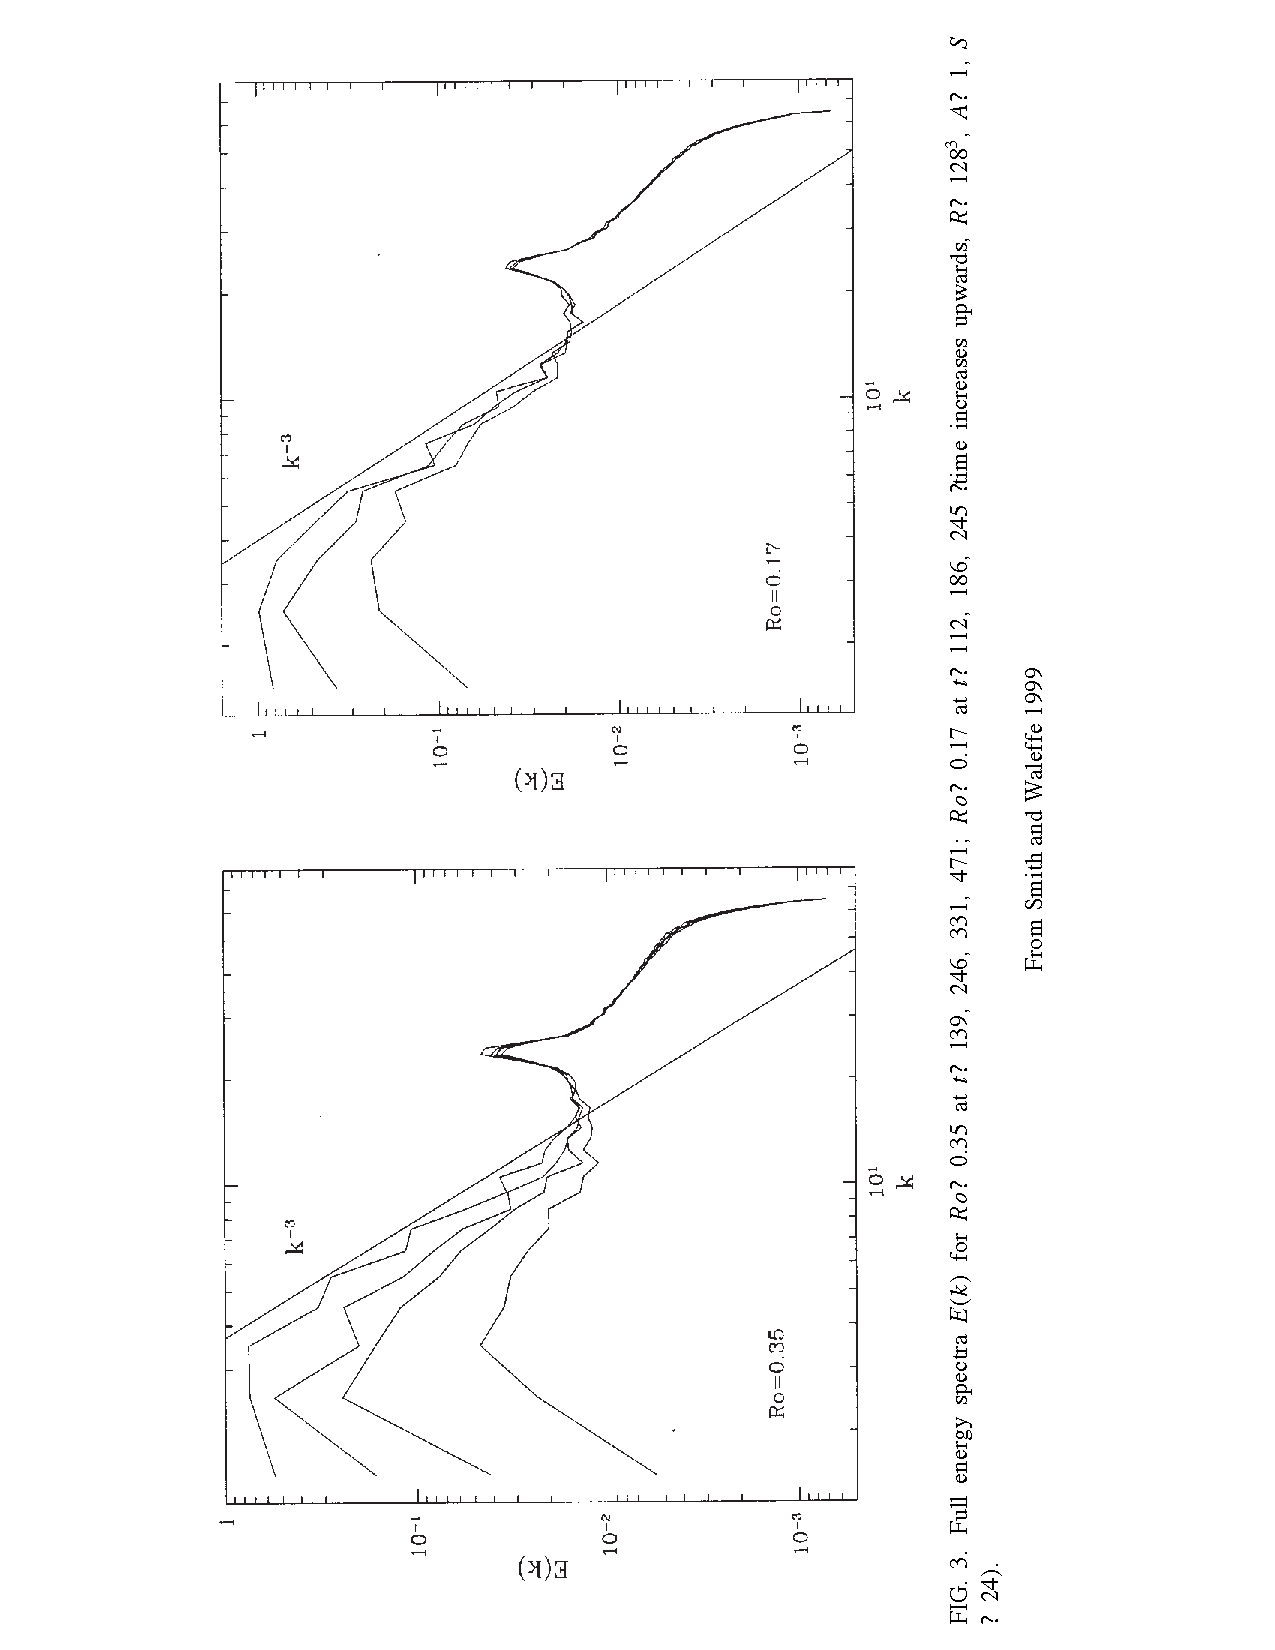
\includegraphics[angle=-90,width=6.in]{SW99Fig3}
\caption{From Smith and Waleffe 1999}
\label{fig:SW99Fig3}
\end{center}
\end{figure}
\begin{figure}
\begin{center}
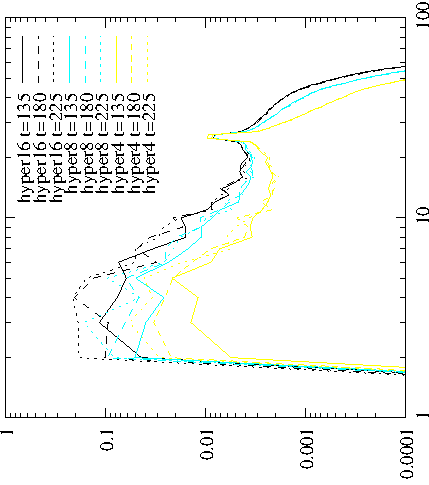
\includegraphics[angle=-90,width=6.in]{r16ketime}
\caption{From sandia/lanl dns code for different kinds of hypeviscosity}
\label{fig:r16ketime}
\end{center}
\end{figure}



\begin{figure}
\begin{center}
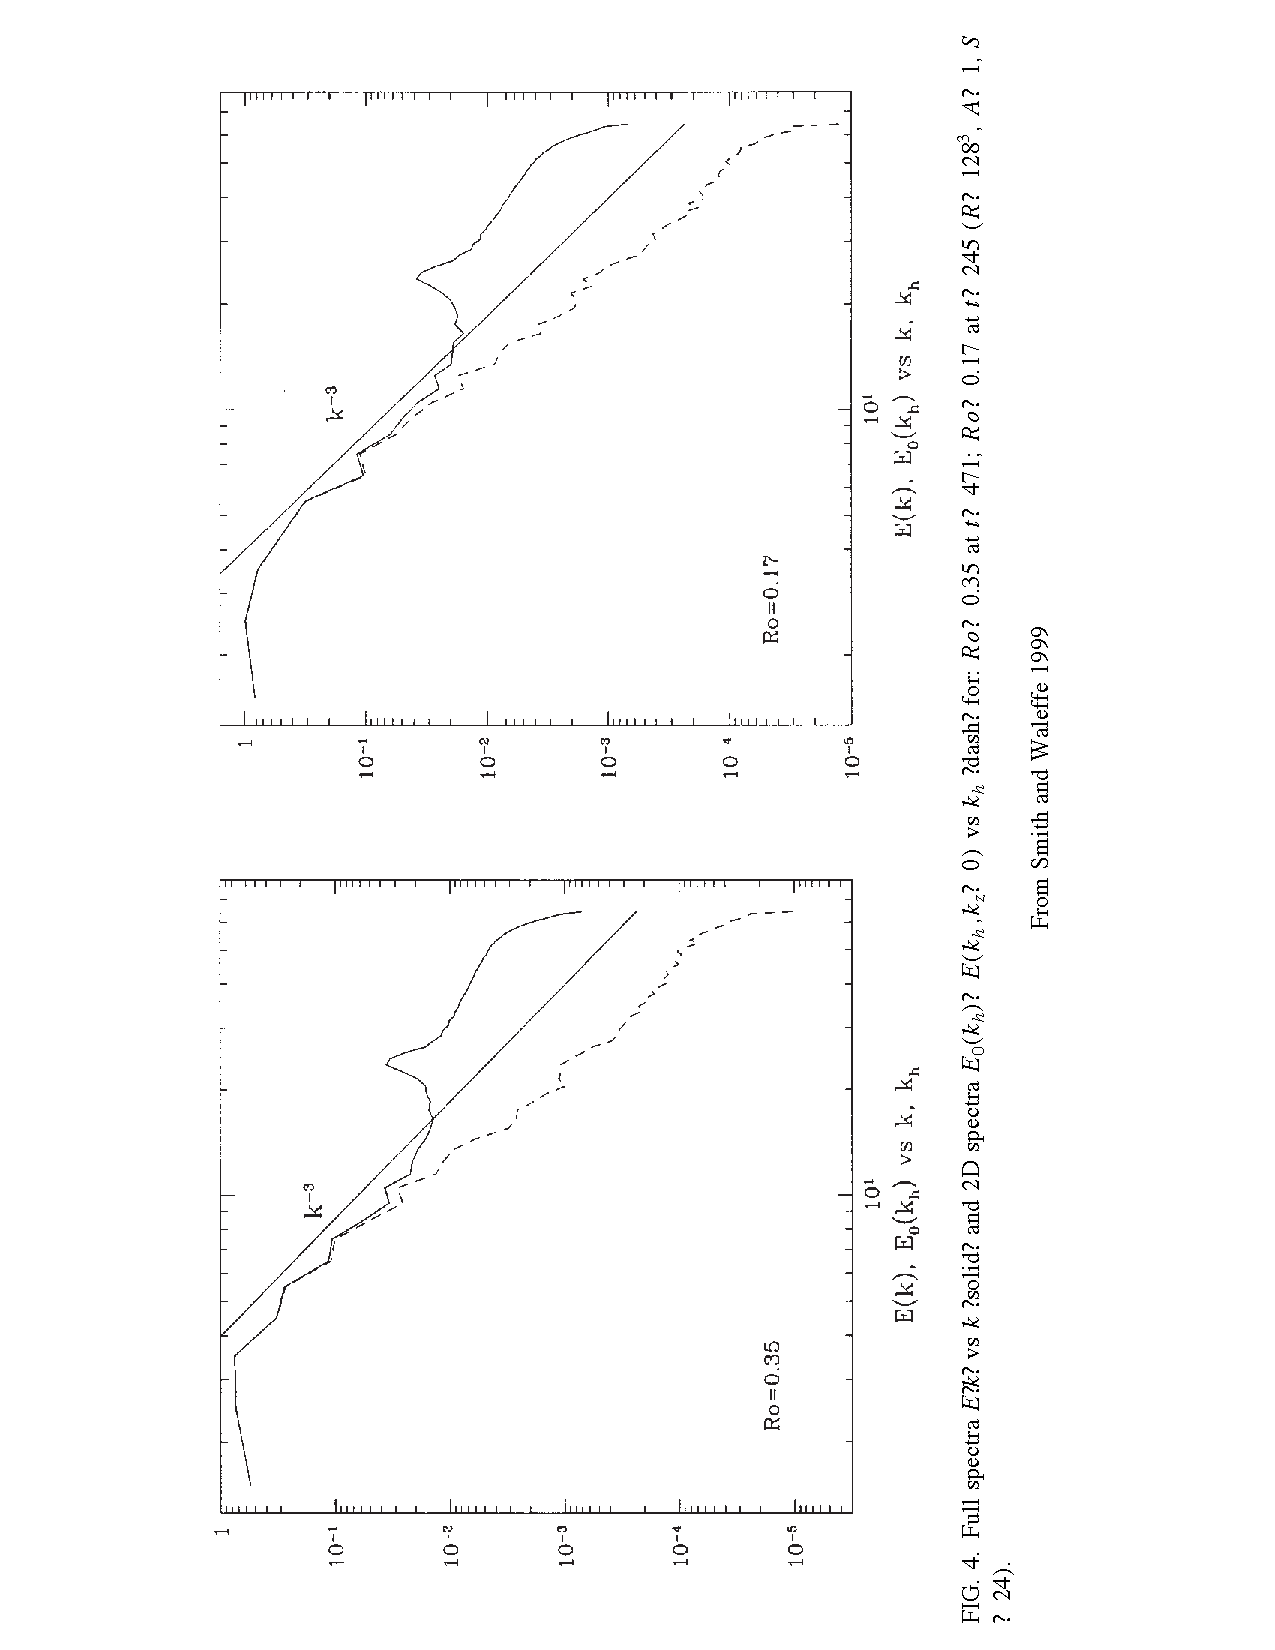
\includegraphics[angle=-90,width=6.in]{SW99Fig4}
\caption{From Smith and Waleffe 1999}
\label{fig:SW99Fig4}
\end{center}
\end{figure}

\begin{figure}
\begin{center}
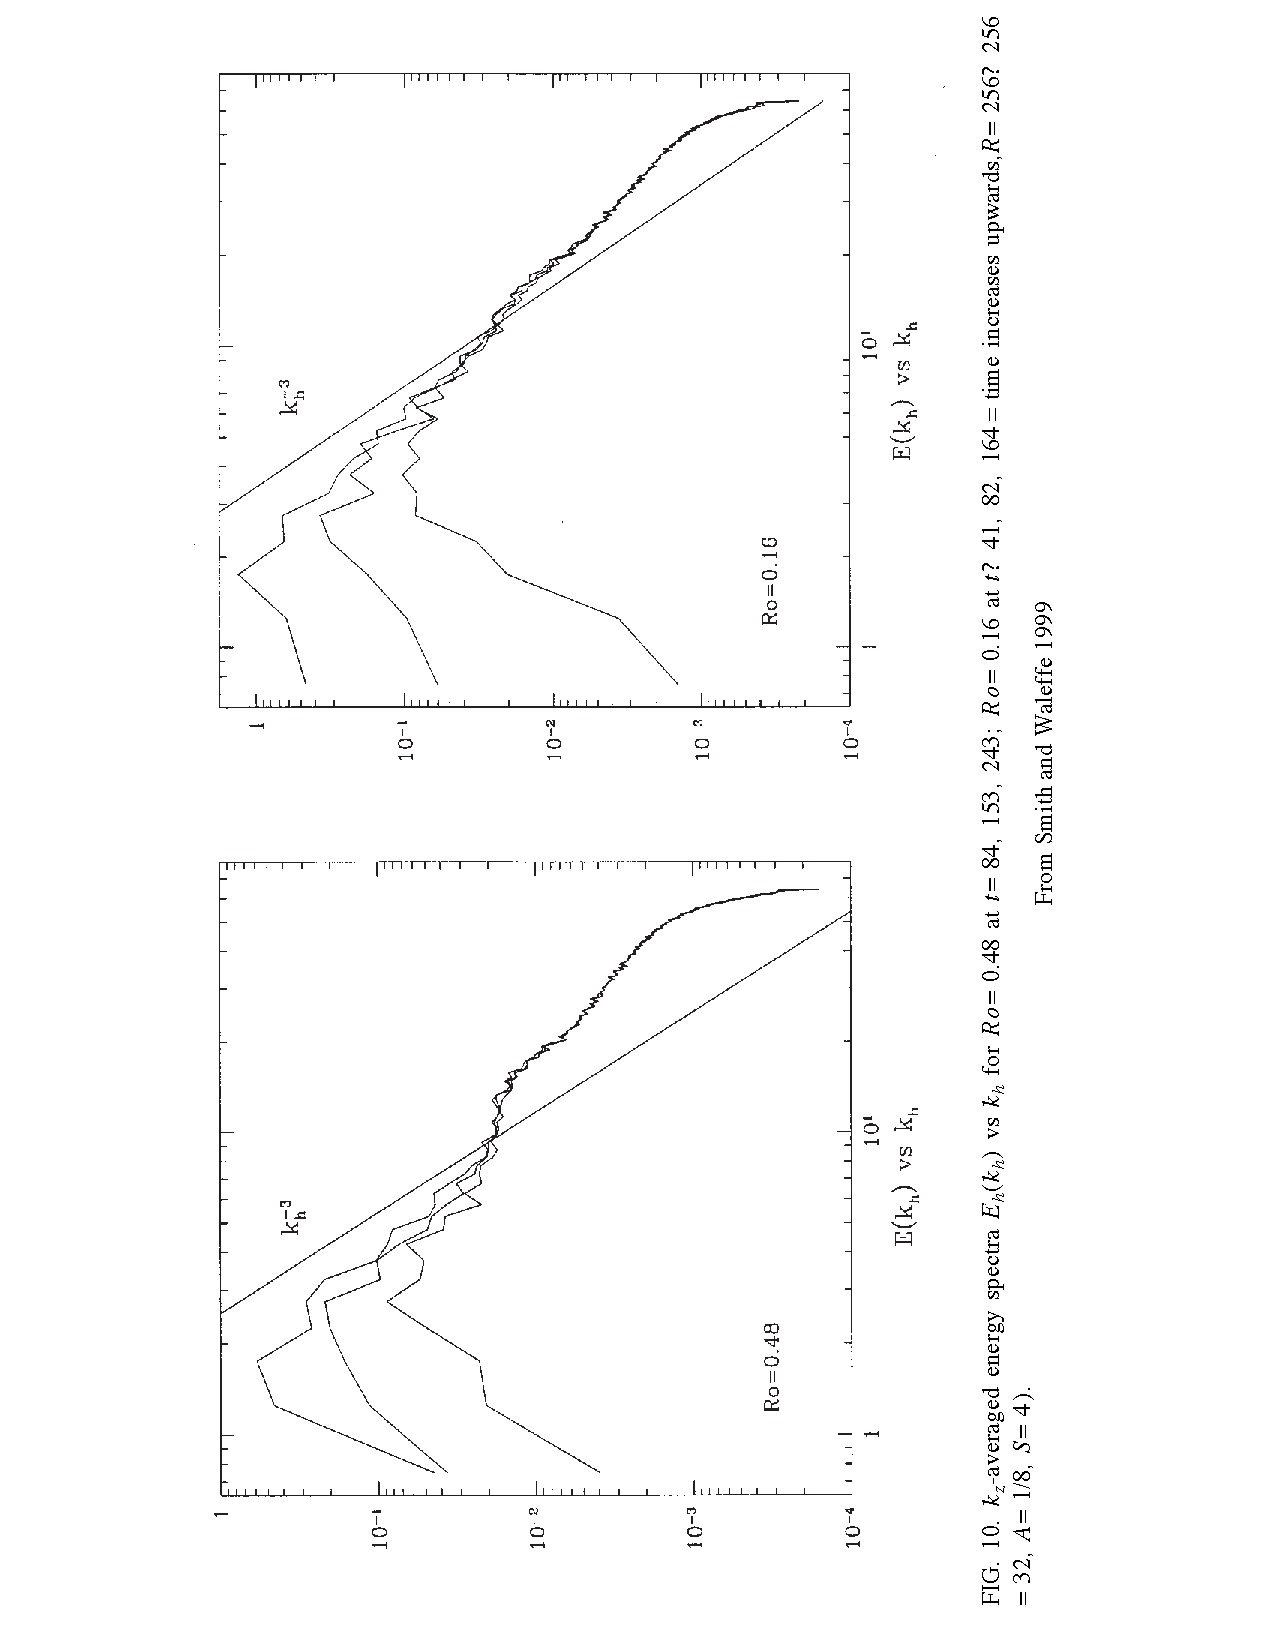
\includegraphics[angle=-90,width=6.in]{SW99Fig10}
\caption{From Smith and Waleffe 1999}
\label{fig:SW99Fig10}
\end{center}
\end{figure}


\subsection{Test of stratification only, $fcor=0$ (no rotation) }

Compare figure (\ref{fig:SW02Fig2}) to figure (\ref{fig:t900})

\begin{figure}
\begin{center}
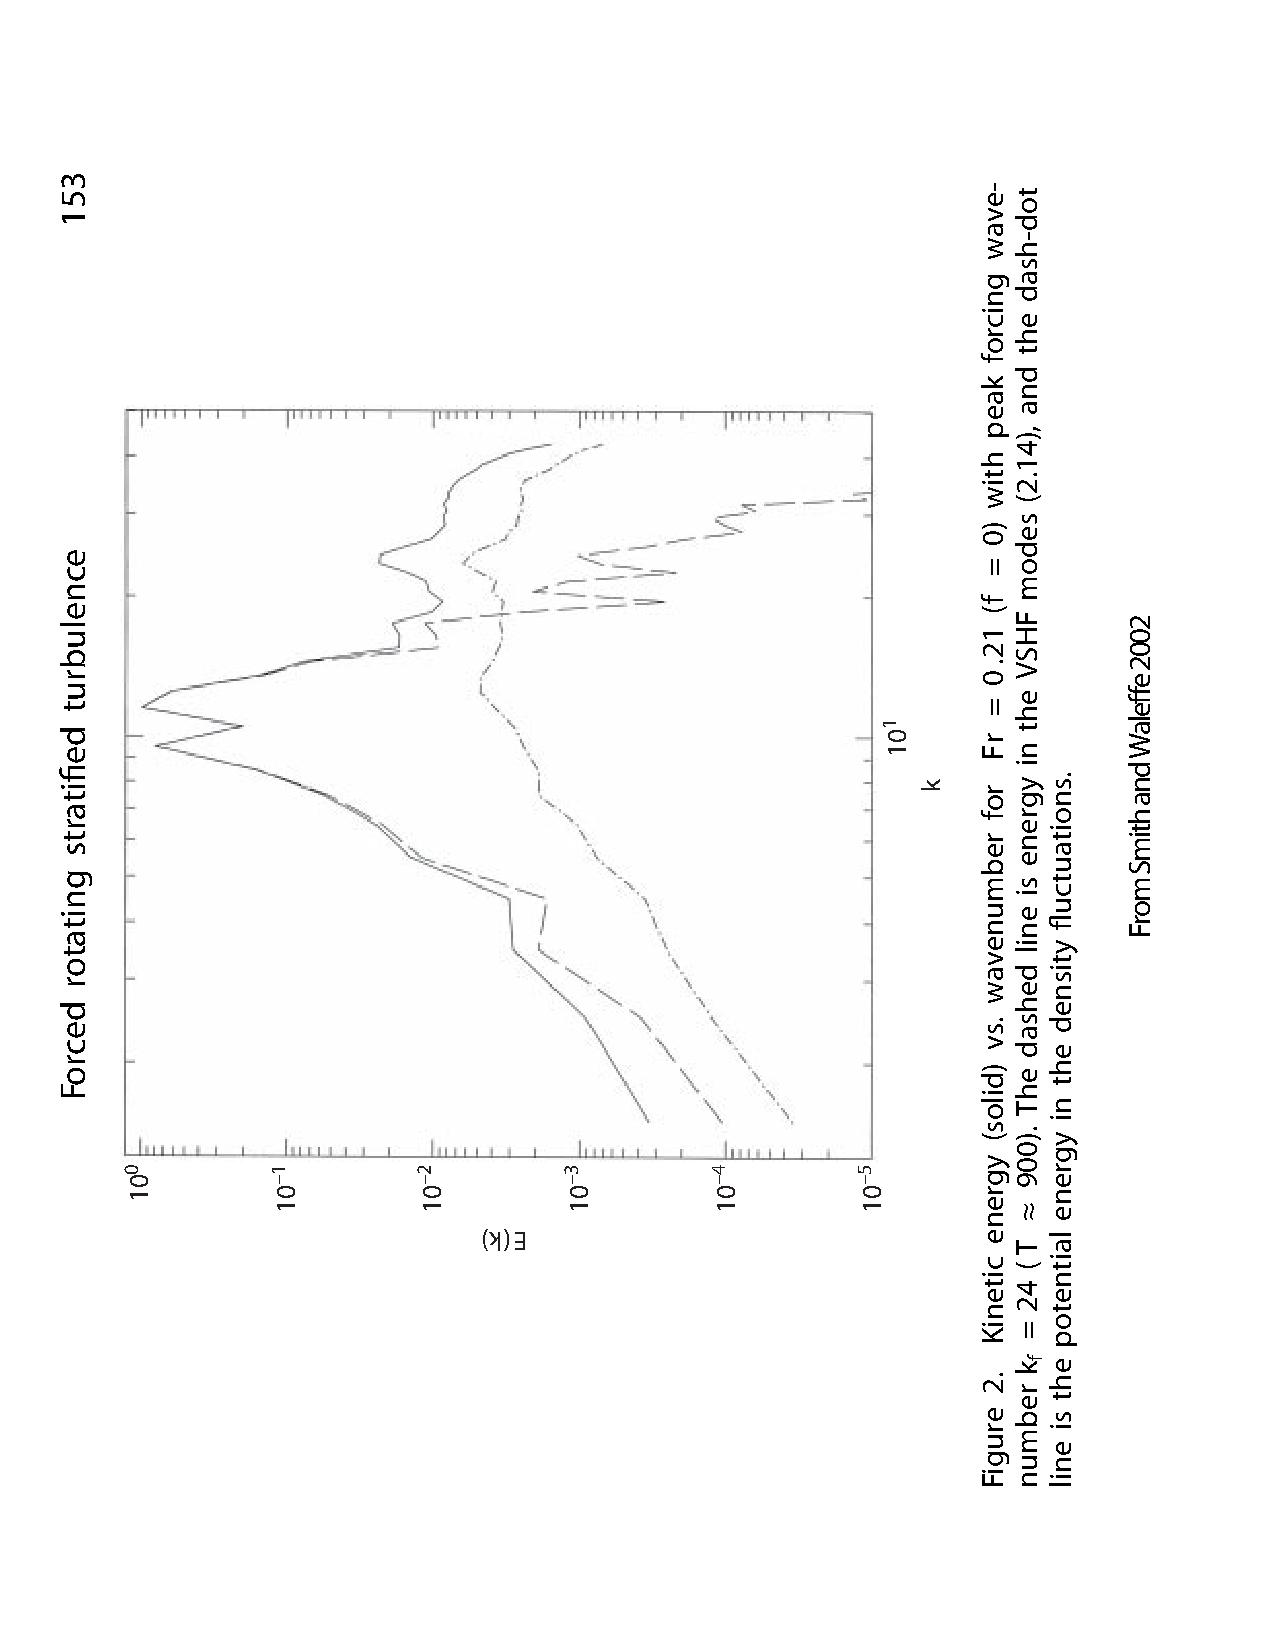
\includegraphics[angle=-90,width=6.in]{SW02Fig2}
\caption{From Smith and Waleffe 2002}
\label{fig:SW02Fig2}
\end{center}
\end{figure}
\begin{figure}
\begin{center}
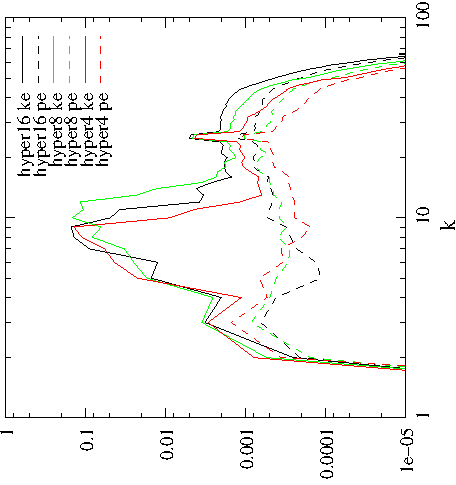
\includegraphics[angle=-90,width=4.in]{t900}
\caption{From the sandia/lanl dns code for 3 different types of hyperviscosity.}
\label{fig:t900}
\end{center}
\end{figure}





First test, $f=0, N\ne0$. Choose $bous=107.08$ with hyperviscosity. Then
\begin{equation}
Fr = \frac{\left((.5)(2 \pi 24)^{2}\right)^{1/3}}{107.08}= .21
\end{equation} 
Forcing is: 
\begin{verbatim}
sto_high_24.
\end{verbatim}
A plot of the spectrum is in Figure \ref{fig:norot} and should be
compared to SW02's Figure 2.
\begin{figure}
\begin{center}
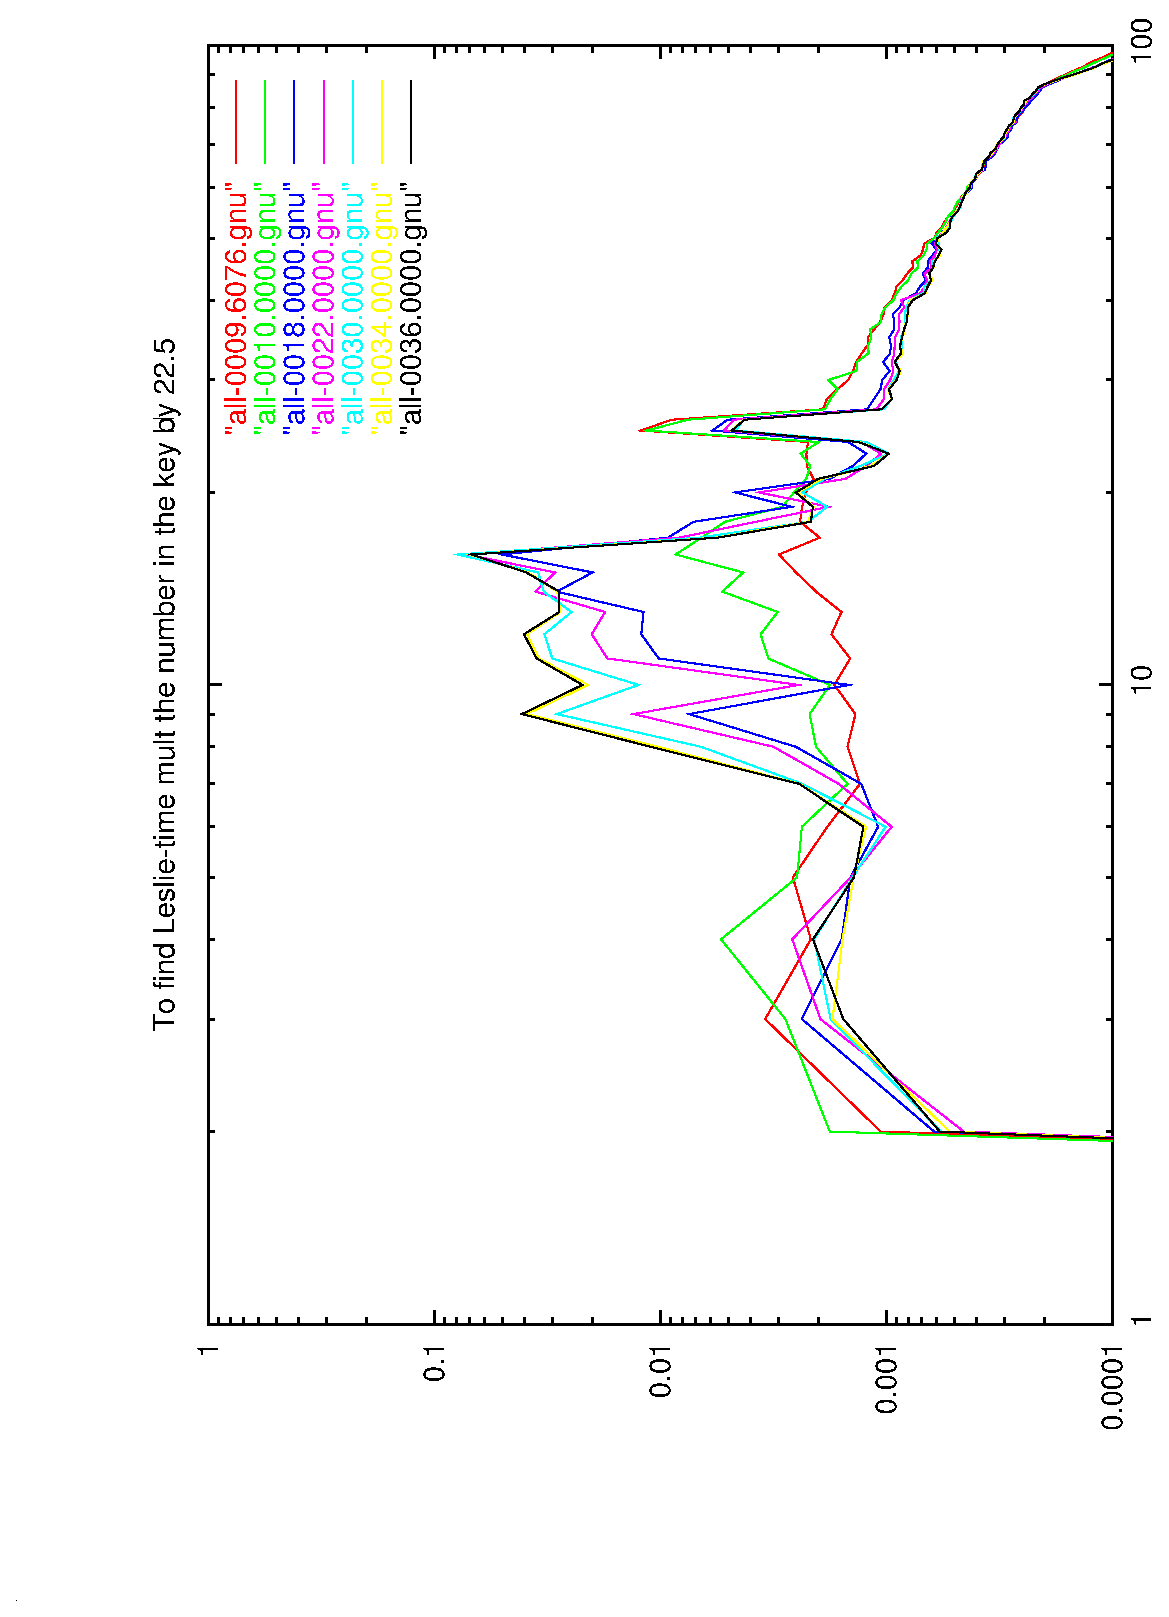
\includegraphics[angle=-90,width=6.in]{frp21}
\caption{Spectrum from $200^3$ simulation of LANL/Sandia DNS code with
  no rotation and $Fr=.21$. This is Smith and Waleffe 2002 Figure 3.}
\label{fig:norot}
\end{center}
\end{figure}

\subsection{Test of nontrivial rotation and stratification $N\ne0, f\ne0$ - }

\begin{figure}
\begin{center}
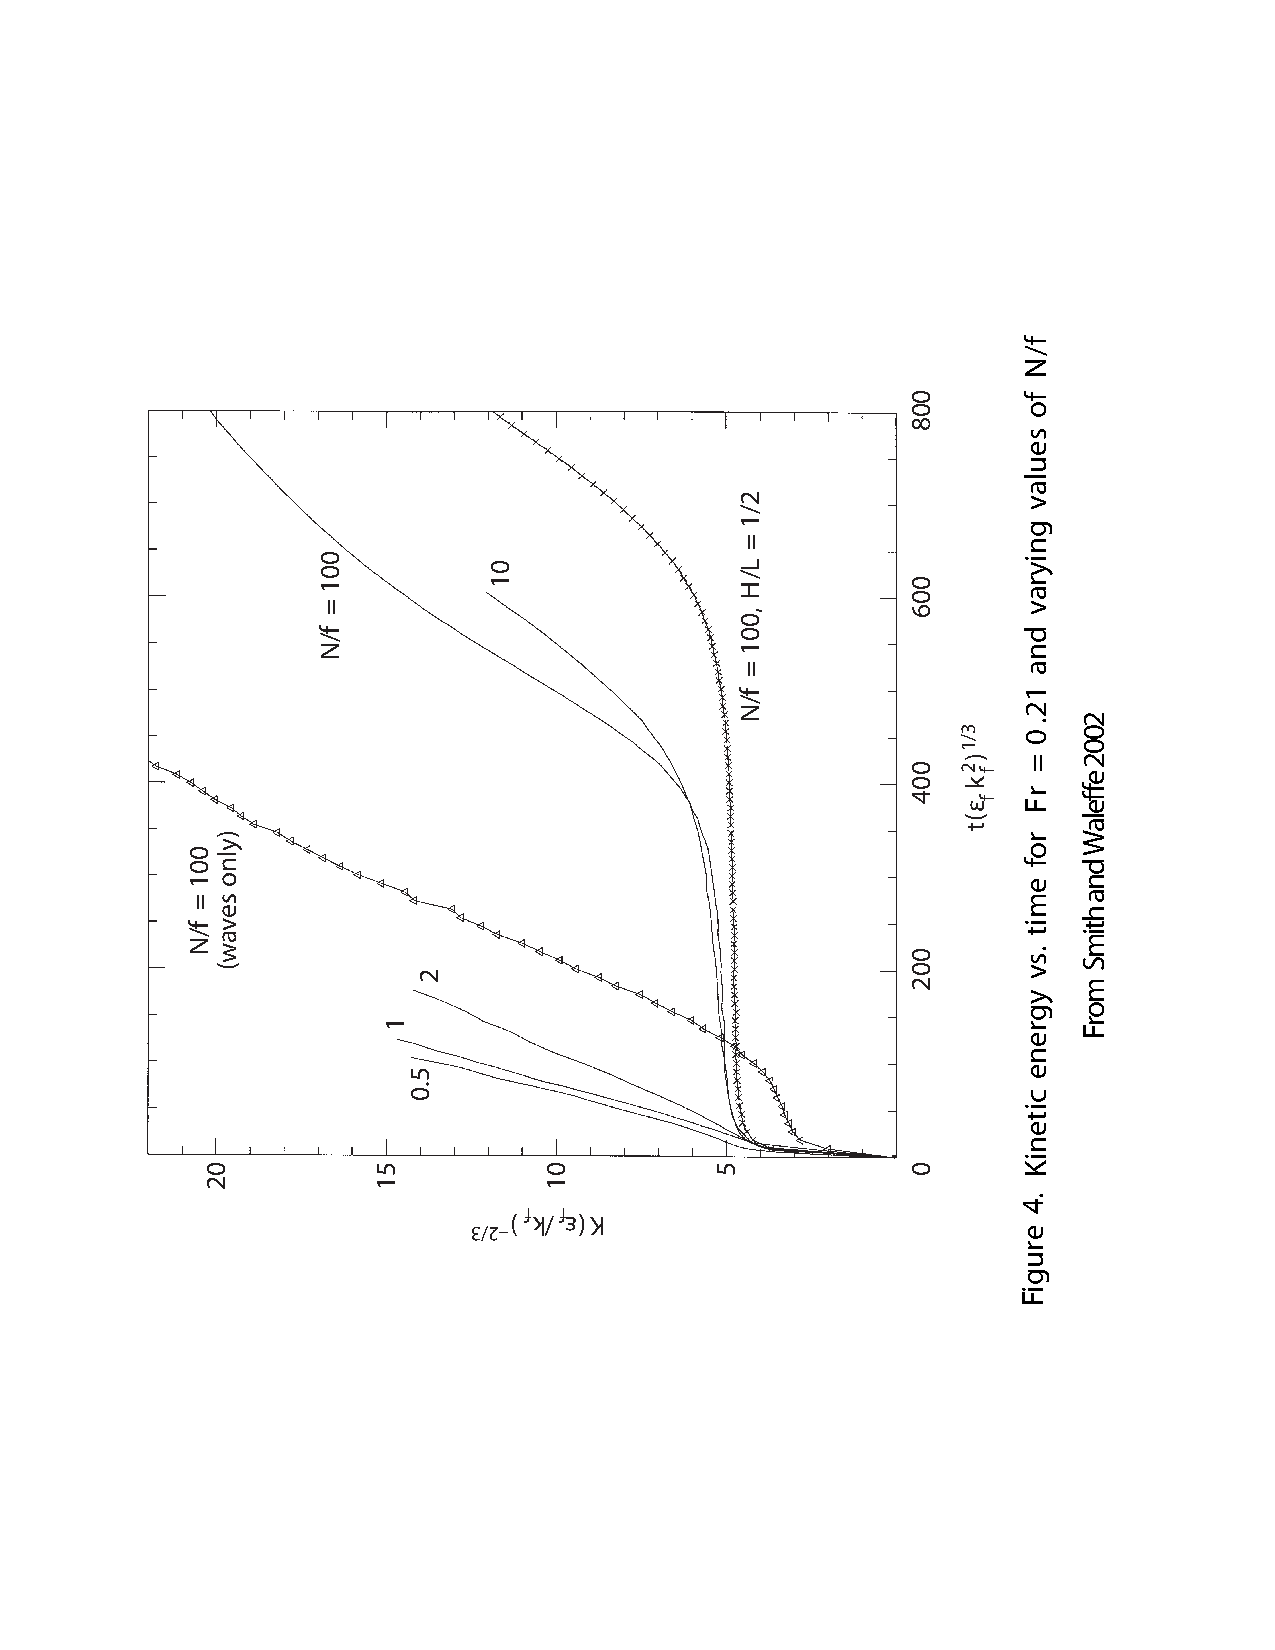
\includegraphics[angle=-90,width=6.in]{SW02Fig4}
\caption{From Smith and Waleffe 2002}
\label{fig:SW02Fig4}
\end{center}
\end{figure}

\begin{figure}
\begin{center}
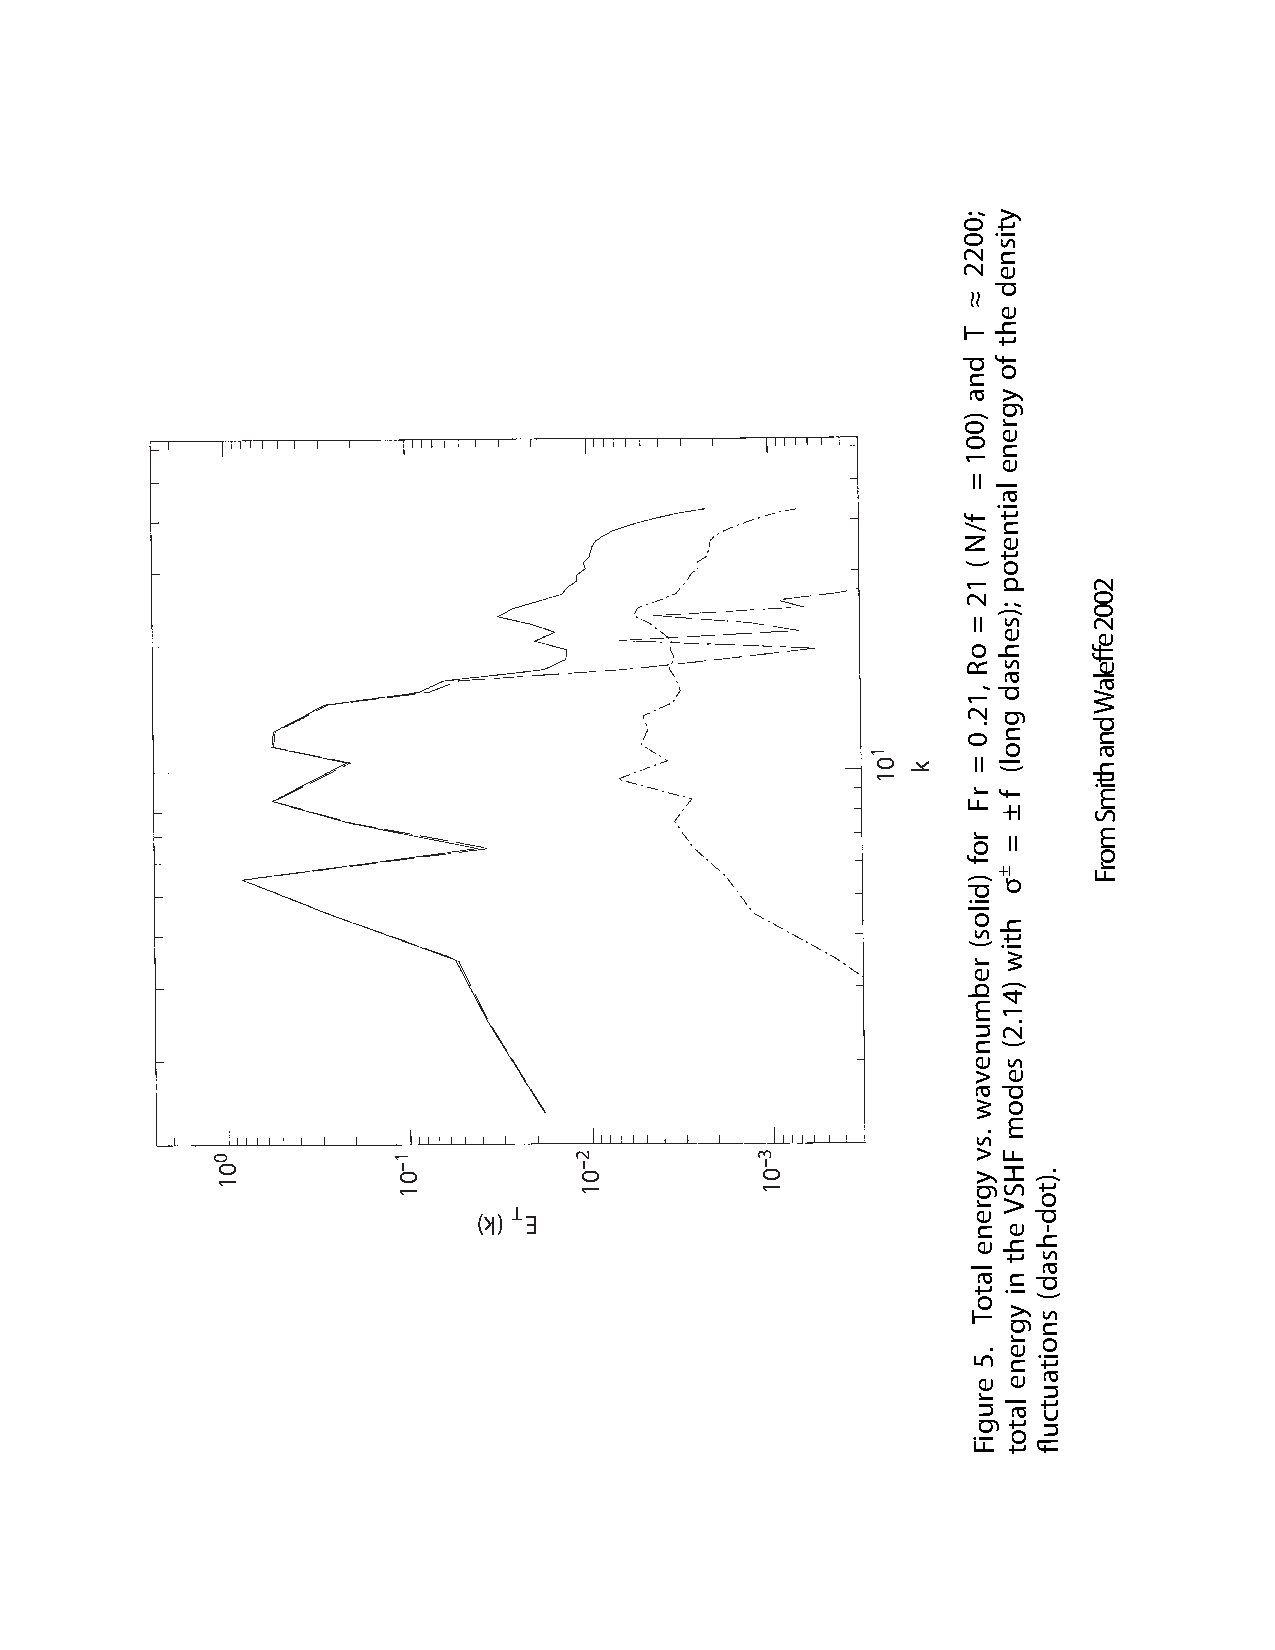
\includegraphics[angle=-90,width=4.in]{SW02Fig5}
\caption{From Smith and Waleffe 2002}
\label{fig:SW02Fig5}
\end{center}
\end{figure}


\begin{eqnarray}
Fr &=& \frac{\left((.5)(2 \pi 24)^{2}\right)^{1/3}}{107.08}= .21 \\ 
Ro &=& \frac{\left((.5)(2 \pi 24)^{2}\right)^{1/3}}{1.07077} = 21
\end{eqnarray} 
This means $\text{bous}=108.07$ and $\text{fcor} =1.07077 $ . We try
to produce the plots in Smith and Waleffe Figure 4 and 5.

Forcing is
\begin{verbatim}
sto_high_24.
\end{verbatim}


\section{Bousinesq scalars we're interested in computing}

We'd like to compute the following (dimensional) quantities integrated
around in the volume:

\begin{itemize}
\item[1.] Total energy and total energy dissipation

\begin{equation}
\frac{\partial}{\partial t} \frac{1}{2} \int_V  
         \left[  (u^2 + v^2 + w^2) +   \theta^2\right]  
= \frac{1}{2}\int_V \left[  \nu \nabla^2 (u^2 + v^2 + w^2)  
                     + \kappa \nabla^2 \theta^2
                         \right] 
\end{equation}

\item[2.] Potential energy, $\frac{1}{2} \theta^2$ 

\item[3.] Kinetic energy, $\frac{1}{2} ( u^2 + v^2 + w^2 )$ 
  
\item[4.] Potential vorticity (q) and its production-dissipation which
  should globally integrate to zero I think.
  \begin{equation}
  \frac{\partial}{\partial t} \int_V   
           \left[ q \right]  
  = \int_V \left[ \nu (\nabla^2 \mathbf\omega) \cdot \mathbf{\nabla}
    (\bar{\theta})
                       + \kappa (\nabla^2 \mathbf{\nabla} \theta) \cdot  
                       (\mathbf\omega  
                       + \text{fcor} ~{\bf{\hat{z}}} ))  
                           \right]  
  \end{equation}
  
  Here $\mathbf = \mathbf\nabla \times \mathbf u$ is the vorticity and
  $\bar\theta = \theta_o -\text{bous}~ z + \theta(x,y,z)$. Also, $q =
  (\mathbf\omega + \text{fcor}~\mathbf{\hat{z}}) \cdot \mathbf\nabla
  \bar\theta.$

\item[5.] Potential enstrophy $Q = q^2/2$ and its
  production-dissipation. This is the important production-dissipation
  rate we need for our two-point correlation.

\item[6.] Potential vorticity production-dissipation

\item[7.] Potential enstrophy
  \begin{equation} 
    \frac{\partial}{\partial t} \int_V   \left[ Q \right]   
    = \int_V \left[ \nu  ~q (~\nabla^2 ~\mathbf\omega) \cdot \mathbf{\nabla}
      (\bar{\theta})   
      + \kappa  ~q ~\nabla^2 (\mathbf{\nabla} \theta) \cdot  
      (\mathbf\omega   
      + \text{fcor} ~{\bf{\hat{z}}} ))   
    \right]   
  \end{equation} 

\item[8.] two-point correlation (coming)

\end{itemize}

\section{Comparing SW to KSW}
In the two-point correlation paper the equations we use are scaled
differently than than we use in Mark's code (which are the same
equations used in SW). To make comparisions with our results in the
two-point correlation paper we have to keep in mind the following
scalings. Note, these are relationships between {\sl{dimensional}}
quantities, not nondimensional quantities.
\begin{gather}
\tilde\rho = (\frac{b \rho_o}{g})^{1/2} ~\theta\\
(\frac{g}{\rho_o b})^{1/2}~\rho = (\frac{g \rho_o}{b}) - \text{bous}
~z + \theta = \bar\theta \\
N = \text{bous} = (\frac{g b}{\rho_o})^{1/2}\\
pe_{\text{ksw}} = \frac{1}{2} \theta^2 = \frac{g}{\rho_o b} \tilde\rho^2\\
q_{\text{ksw}} = (\frac{g}{b \rho_o})^{1/2} q_{\text{SW}}
\end{gather}

\end{document}
